\chapter{Stato dell'arte}\label{ch:background}
Il capitolo introduce teorie e tecniche alla base del lavoro svolto. \`E opportuno premettere che quanto verrà descritto nel seguito rappresenta un sottoinsieme eterogeneo all'interno del mondo del Machine Learning, sia dal punto di vista cronologico che da quello modellistico, che però trova una sintesi nei modelli sviluppati. La trattazione procede dunque secondo una suddivisione concettuale che guarda principalmente ai modelli ed ai domini applicativi.

Il paragrafo \ref{sec:intro:MLeNN} descrive i principi del Machine Learning ed introduce le Reti Neurali Artificiali come modello computazionale, presentando alcune delle tecniche adottate nel loro utilizzo.

Il paragrafo~\ref{sec:intro:cnn} introduce l'approccio costruttivo nell'allenamento delle Reti Neurali e descrive l'algoritmo Cascade Correlation per lo sviluppo di reti feedforward costruttive.

Nel paragrafo~\ref{sec:intro:rnn} vengono introdotte le Reti Neurali Ricorrenti per il trattamento di sequenze.

Nel paragrafo~\ref{sec:intro:rc} viene presentato il paradigma del Reservoir Computing, delineandone caratteristiche e motivazioni, e vengono introdotte le Echo State Networks nella loro formulazione classica di Reti Neurali Ricorrenti utilizzate per processare sequenze di input.

Il paragrafo~\ref{sec:intro:struct} descrive il problema dell'apprendimento di dati strutturati, indicando alcune delle soluzioni offerte dal paradigma neurale in questo campo.


%%%%%%%%%%%%%%%%%%%%%%%%%%%%%%%%%%%%%%%%%%%%%%%%%%%%%%%%%%%%%%%
%%%%%%%%%%%%%%%%%%%%%%%%%%%%%%%%%%%%%%%%%%%%%%%%%%%%%%%%%%%%%%%
\section{Machine Learning e Reti Neurali}\label{sec:intro:MLeNN}
Il Machine Learning \cite{Mitchell:ML, Hastie:EOSL} è un settore dell'Informatica che propone metodi ed algoritmi per l'apprendimento e la predizione, ovvero mirati ad apprendere da esempi un compito computazionale definito. I modelli di Machine Learning hanno il compito di risolvere problemi del mondo reale difficili da trattare con tecniche tradizionali e si configurano come strumenti complementari rispetto ai modelli analitici basati sulla conoscenza pregressa, agli algoritmi propri della programmazione imperativa o all'Intelligenza Artificiale classica.
Obiettivo del Machine Learning è dunque far sì che l'esperienza (collezione di esempi) possa essere appresa in maniera automatica per risolvere un compito, in modo da costruire dei \emph{modelli} (o \emph{ipotesi}) utili per poter fare predizioni. In altri termini, possiamo dire che il Machine Learning studia e propone metodi per inferire dipendenze (o funzioni, o ipotesi), da esempi di dati osservati, che siano in grado di approssimare i dati noti (\emph{fitting}) e che siano capaci di \emph{generalizzare}, ovvero rispondere in modo accurato per dati nuovi. 

% apprendimento come ricerca di una funzione nello spazio delle ipotesi
I modelli di Machine Learning hanno dunque lo scopo di catturare le relazioni tra i dati e definiscono la classe di funzioni che il sistema può calcolare (\emph{spazio delle ipotesi}). L'apprendimento (\emph{learning}) avviene modificando i parametri liberi di un modello in modo da trovare, all'interno dello spazio delle ipotesi, una funzione che possa correttamente approssimare la \emph{funzione obiettivo} (non nota) in modo da poter essere usata per fare predizioni su nuovi dati di input. 

Distinguiamo due tipologie di problemi, o \emph{task}, che i modelli di Machine Learning si propongono di affrontare: task di apprendimento \emph{supervisionato} e di apprendimento \emph{non-supervisionato}. \\
% apprendimento supervisionato (classificazione e regressione)
Nel primo caso la sorgente di esperienza per la funzione obiettivo $f_t$ è rappresentata da un dataset contenente un insieme di coppie, o \emph{esempi etichettati}
\[ D = \lbrace (x_i, d_i) \rbrace_{i=1}^{l} \]
dove $x$ è un input e $d$ è un valore di output atteso, o \emph{target}, dato da un \emph{teacher} in accordo ad $f_t(x)$.
Nel contesto dell'apprendimento supervisionato è inoltre possibile un'ulteriore suddivisione: si parla di \emph{classificazione} nel caso di funzioni obiettivo a valori discreti, tali che $f_t(x)$ restituisce il valore della classe di appartenenza dell'input $x$, mentre sono task di \emph{regressione} quelli in cui la funzione obiettivo abbia valori reali, in $\R$ o $\R^n$.\\
% apprendimento non-supervisionato
Nel caso dell'apprendimento non-supervisionato la sorgente di esperienza è invece caratterizzata dalla mancanza di valori target, il dataset usato per allenare un modello è quindi composto da soli esempi non etichettati:
\[ D = \lbrace (x_i) \rbrace_{i=1}^{l} \]
L'obiettivo è in questo caso quello di trovare \emph{raggruppamenti naturali} in un insieme di dati. L'apprendimento non-supervisionato viene utilizzato tipicamente per fare clustering, riduzione della dimensionalità dei dati, visualizzazione e preprocessing, modellazione della densità dei dati.


Tutti i task ed i modelli che verranno discussi nel corso della tesi si riferiscono a casi di apprendimento \emph{supervisionato}, affrontati in particolare ricorrendo al paradigma neurale, ovvero attraverso modelli di Reti Neurali Artificiali.


%%%%%%%%%%%%%%%%%%%%%%%%%%%%%%%%%%%%%%%%%%%
\subsection{Reti Neurali Artificiali}\label{intro:ann}
Le Reti Neurali Artificiali \cite{Haykin:NN,Bishop:NNFPR} sono un vasto insieme di modelli di Machine Learning, sviluppati secondo un'analogia --- più o meno marcata~--- con le strutture e le dinamiche che si ritrovano nel cervello. Reti di questo tipo sono infatti formate da più unità (neuroni), collegate fra loro tramite connessioni pesate (sinapsi). La relazione tra ingresso ed uscita della rete è dunque determinata dalla propagazione del segnale di input sulle connessioni ed attraverso le unità.
In analogia con il modello biologico, un singolo neurone artificiale ha un'uscita, o \emph{attivazione}, che dipende dai segnali in ingresso, corrispondenti alle attivazioni di altre unità:
\begin{equation}\label{eq:intro:neurone}
o(\vect{x}) = f( \sum_{j} w_{j} x_{j} )
\end{equation}
dove $x_j$ indica il $j$-esimo input, parte del segnale di ingresso $\vect{x}$, $w_{j}$ indica il peso assegnato alla connessione corrispondente ed $f$ è detta \emph{funzione di attivazione}.  

% Multilayer Perceptron
Nonostante la semplicità di un singolo neurone artificiale, la composizione di più unità permette la creazione di modelli computazionalmente molto potenti e flessibili: è il caso del Multilayer Perceptron \cite{Bishop:NNFPR,Haykin:NN}, che rappresenta certamente uno dei modelli più utilizzati nell'ambito del Machine Learning.
Reti di questo tipo sono realizzate componendo più livelli, o \emph{layer}, di unità collegate secondo una topologia aciclica (i.e.\ Reti Neurali Feedforward): il segnale viene quindi fatto passare da un layer di input ad uno o più livelli, detti \textit{nascosti}, fino ad un livello di output, le cui attivazioni vengono usate per determinare l'uscita della rete. La funzione, o ipotesi, realizzata da un Multilayer Perceptron con un layer nascosto è 
\begin{equation}\label{eq:intro:mlp}
h(\mathbf{x}) = f_{p} (  \sum_{j} w_{pj} f_{j} ( \sum_{i} w_{ji} x_{i} ) )
\end{equation}
dove $f_p$ ed $f_j$ sono rispettivamente le funzioni di attivazione delle unità di output e delle unità nascoste e $w_{rs}$ indica il peso sulla connessione che va dall'unità $s$-esima verso l'unità $r$-esima. La figura~\ref{fig:intro:mlp} mostra l'architettura aciclica di un Multilayer Perceptron con un unico layer nascosto.
\begin{figure}[tbp]
\centering
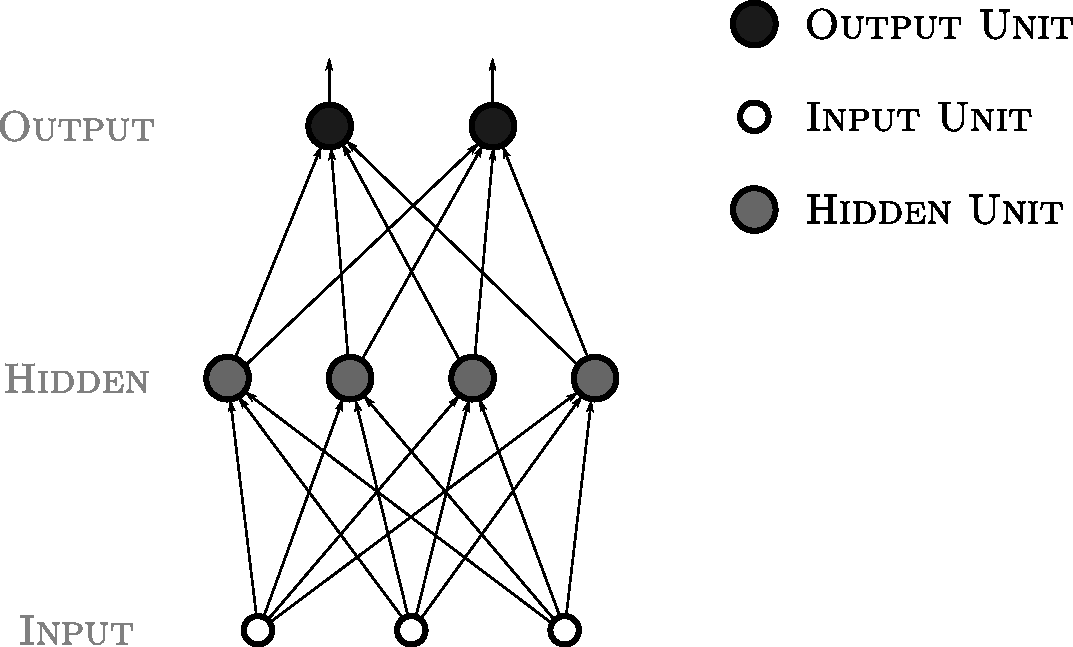
\includegraphics[width=0.7\columnwidth]{img/mlp}
\medskip
\caption[Multilayer Perceptron.]{Multilayer Perceptron. Architettura di una rete con 3 unità input, 2 unità di output e 4 unità nascoste, in un unico layer.}
\label{fig:intro:mlp}
\end{figure}

Come si vede dalle equazioni (\ref{eq:intro:neurone}) e (\ref{eq:intro:mlp}), i \emph{parametri liberi} di una Rete Neurale Artificiale sono rappresentati dai pesi, a valori reali, sulle connessioni: lo spazio delle ipotesi è dunque in questo caso continuo, il che permette di ascrivere il paradigma neurale alla classe degli approcci \emph{sub-simbolici} nel campo del Machine Learning. Sono invece detti \emph{iperparametri} di un modello i fattori che ne determinano lo spazio delle ipotesi (e.g.\ il numero di unità nascoste) o che influenzano l'apprendimento (e.g.\ i parametri dell'algoritmo di learning utilizzato).

Modelli di questo tipo si caratterizzano per la capacità di trattare efficacemente dati sia continui che discreti, realizzando task di classificazione o regressione, e mostrando tolleranza rispetto a dati di input rumorosi o incompleti.
La presenza di almeno un layer nascosto di unità con funzioni di attivazione non lineari (tipicamente sigmoidali, e.g.\ $\tanh$) ha inoltre l'effetto di rendere il Multilayer Perceptron un \emph{approssimatore universale} \cite{Cybenko:ApproximationBySuperpositions}, in grado cioè di approssimare con precisione arbitraria qualsiasi funzione continua definita su un sottoinsieme compatto di $\R^n$. 

L'apprendimento avviene generalmente, nelle Reti Neurali Feedforward, attraverso l'algoritmo di Backpropagation \cite{Haykin:NN}, che sfrutta una discesa del gradiente per modificare iterativamente i pesi di tutte le connessioni, minimizzando l'errore commesso sugli esempi etichettati di training. 


%%%%%%%%%%%%%%%%%%%%%%%%%%%%%%%%%%%%%%%%%%%
\subsection{Validazione}\label{intro:validazione}
Come detto in precedenza, lo scopo del processo di apprendimento in un modello di Machine Learning è quello di trovare una buona approssimazione, a partire da dati noti, all'interno di uno spazio di funzioni. Per definire cosa si intenda per \emph{buona} è necessario riferirsi alla capacità di \emph{generalizzazione}, ovvero all'accuratezza nel fare previsioni su dati sconosciuti.
La generalizzazione è dunque un punto determinante del Machine Learning e viene esplorata durante una fase di test in cui si esegue la valutazione dell'ipotesi in termini di capacità predittiva.

Per poter valutare la qualità dell'approssimazione di un modello si ricorre a delle funzioni di \emph{loss}
\begin{equation}
L(h(x), d) 
\end{equation}
che misurano la discrepanza tra l'output del modello ed il valore desiderato $d$ su un campione $x$ in ingresso (i.e.\ valori alti della loss indicano scarsa approssimazione).
Per i task di apprendimento supervisionato consideriamo le seguenti funzioni di loss:
\begin{itemize}
\item Classificazione: \emph{errore di classificazione}
\begin{equation}
L(h(x_i), d_i) =  
\begin{cases}
0 & \text{se } h(x_i) = d_i \\
1 & \text{altrimenti}
\end{cases}
\end{equation}
\item Regressione: \emph{errore quadratico}
\begin{equation}
L(h(x_i), d_i) =  (d_i - h(x_i))^2
\end{equation}
\end{itemize}

Il legame tra funzione di loss e generalizzazione è determinato dall'\emph{ipotesi dell'apprendimento induttivo}, secondo cui ogni ipotesi $h$ che approssima bene $f_t$ sugli esempi di training approssimerà bene $f_t$ anche su (nuove) istanze sconosciute di input.

Tale assunzione è fondante dell'approccio che si adotta nella realizzazione dell'apprendimento.
In accordo con tale ipotesi, per determinare l'approssimazione migliore di $f_t$, si ricerca quindi un'ipotesi $h$ che minimizzi l'\emph{errore reale} $R$
\begin{equation}
R = \int L(d, h(x))\, dP(x,d)  
\end{equation}
dove $d$ è un valore dato dal teacher, $P(x,d)$ è la distribuzione dei dati --- che generalmente non è nota a priori --- e $L(d, h(x))$ è una funzione di loss.\\
Disponendo solo di un insieme finito di dati di training
\begin{equation} 
D = \lbrace (x_i, d_i) \rbrace_{i=1}^{l}  
\end{equation}
per cercare $h$ si ricorre alla minimizzazione del \emph{rischio empirico} (errore di training), alla ricerca dei migliori valori per i parametri liberi del modello
\begin{equation}
R_{emp} = \frac{1}{l} \sum_{i} L(d_i, h(x_i))
\end{equation}
seguendo il principio induttivo della \emph{Minimizzazione del Rischio Empirico}.

Esiste tuttavia la possibilità che l'ipotesi dell'apprendimento induttivo non sia fondata, in particolare nel caso di \emph{overfitting}.
Considerando un'ipotesi generica $h_i \in H$ e chiamando $\epsilon_i$ il suo errore reale e $E_i$ il suo errore empirico, diciamo che un learner fa \emph{overfitting} se l'ipotesi in output $h_{out}$ è tale che esiste una ipotesi diversa $h_j \in H$ per cui: $E_{out} < E_j$ e $\epsilon_{out} > \epsilon_j $.
Intuitivamente, quindi, l'overfitting corrisponde alla situazione in cui un modello sia stato allenato fino a raggiungere un livello di approssimazione dei dati di training eccessivamente alto, perdendo di conseguenza la capacità di generalizzare.

In modo particolare nell'uso di Reti Neurali, caratterizzate da un'estrema flessibilità nell'approssimare la funzione obiettivo, si rende dunque necessario un procedimento che permetta di valutare con accuratezza la performance di un modello. Nel seguito vengono brevemente descritte alcune delle tecniche comunemente usate a questo scopo (si veda anche \cite{Hastie:EOSL}).

\subsubsection*{Hold-out}
Questa tecnica può essere utilizzata qualora si disponga di dataset di grosse dimensioni, e rappresenta il caso più semplice di validazione di un modello.

Il dataset $D$ viene partizionato in due insiemi \emph{disgiunti}: un \emph{training-set} $D_\textup{tr}$ ed un \emph{test-set} $D_\textup{ts} = D \setminus D_\textup{tr}$. Si ha dunque
\[
D = D_\textup{tr} \cup D_\textup{ts} 
% \quad \text{e} \quad D_\textup{tr} \cap D_\textup{ts} = \emptyset
\]
Il modello viene allenato sul training-set e, successivamente, il test-set viene utilizzato per valutarne la capacità di generalizzazione. 

Per garantire che i risultati possano essere rappresentativi della capacità predittiva del modello, il test-set non viene usato per l'adattamento dei parametri liberi né per la selezione del modello (i.e.\ scelta degli iperparametri). A questo scopo, se si hanno maggiori dati a disposizione, è possibile partizionare ulteriormente il training-set, ottenendo un \emph{validation-set} $D_\textup{val}$ che può essere usato per scegliere l'ipotesi migliore. In questo caso, quindi si ha
\[
D = D_\textup{tr} \cup D_\textup{val} \cup D_\textup{ts} 
%\quad \text{e} \quad 
%D_\textup{tr} \cap D_\textup{val} \cap D_\textup{ts} = \emptyset
\]
con i dati in $D_\textup{tr}$ usati per allenare più modelli, $D_\textup{val}$ impiegato per scegliere, fra i vari modelli allenati, quello considerato più adatto al problema affrontato ed, infine, $D_\textup{ts}$ usato per determinare la performance del modello scelto. Il processo di scelta dell'ipotesi migliore attraverso un validation-set è chiamato \emph{model selection} ed avviene dunque secondo un procedimento di \emph{trial and error}.

\subsubsection*{K-fold cross-validation}
Nel caso in cui si abbiano pochi dati a disposizione, l'hold-out può comportare una riduzione eccessiva di dati utili per il training. In questo caso si procede con la variante della \emph{k-fold cross-validation}, che prevede il partizionamento del dataset $D$ in $k$ sottoinsiemi, o \emph{fold}, mutuamente esclusivi
\[
D = D_1 \cup D_2 \cup \dots \cup D_k
%\quad \text{e} \quad 
%D_1 \cap D_2 \cap \dots \cap D_k = \emptyset
\]
Il modello viene dunque allenato e testato per $k$ volte, facendo in modo che la porzione di dati usati per il test non sia usata nel training del modello
\[
D_\textup{tr} = D \setminus D_i
\quad \text{e} \quad 
D_\textup{ts} = D_i
\qquad \text{per} \quad i=1,\dots,k
\]
La performance è infine ottenuta come media delle performance ottenute sul test-set delle varie fold.

L'impiego di k-fold cross-validation consente dunque di usare tutti i dati a disposizione sia per il training che per il test e può essere combinato, come nel caso dell'hold-out, con l'uso di un validation-set per la selezione del modello.

\subsubsection*{Double k-fold cross-validation}
In questo caso vengono realizzati due cicli di cross-validation, di cui quello ``interno'' viene utilizzato per la selezione del modello.

Come per la k-fold cross-validation, il dataset viene inizialmente partizionato in fold
\[
D = D_1 \cup D_2 \cup \dots \cup D_k
%\quad \text{e} \quad 
%D_1 \cap D_2 \cap \dots \cap D_k = \emptyset
\]
e successivamente, ogni fold viene a sua volta suddivisa in $t$ sotto-fold
\[
D_i = D_{i1} \cup D_{i2} \cup \dots \cup D_{it}
%\quad \text{e} \quad 
%D_{i1} \cap D_{i2} \cap \dots \cap D_{it} = \emptyset
\qquad \text{per} \quad i=1,\dots,k
\]
Ogni sotto-fold viene dunque utilizzata per allenare e valutare più iperparametrizzazioni
\[
D_\textup{tr} = D_i \setminus D_{ij}
\quad \text{e} \quad 
D_\textup{val} = D_{ij}
\qquad \text{per} \quad j=1,\dots,t
\]
Tale processo permette di ottenere $k$ modelli ``vincenti'', uno per ogni fold, selezionati in base alla performance media sui validation-set. Il test viene dunque eseguito, su ogni fold, valutando il modello vincente attraverso una k-fold cross-validation
\[
D_\textup{tr} = D \setminus D_i
\quad \text{e} \quad 
D_\textup{ts} = D_i
\qquad \text{per} \quad i=1,\dots,k
\]
La performance del modello è quindi calcolata come la media delle performance raggiunte dalle iperparametrizzazioni vincenti su ogni fold.

La double k-fold cross-validation è un processo accurato, ma computazionalmente dispendioso, che consente di ottenere una stima dell'accuratezza di un modello anche su dataset di dimensioni ridotte. Si distingue tuttavia dalle tecniche precedenti per il fatto di restituire non una, ma $k$, iperparametrizzazioni vincenti.

\subsubsection*{Stratificazione}
Nel partizionare un dataset secondo le tecniche descritte è ovviamente necessario che tutti i sottoinsiemi siano sufficientemente rappresentativi per il problema trattato e che riescano dunque a descrivere le relazioni fra i dati. Eventuali sbilanciamenti nella natura dei dati in uno dei sottoinsiemi possono infatti comportare un \emph{bias} che può avere impatto negativo sulla capacità di generalizzazione dei modelli.

La \emph{stratificazione} è una tecnica mirata ad evitare questo scenario e prevede che i dati vengano partizionati, prima del sampling, in gruppi omogenei, in modo che i sottoinsiemi possano essere formati mantenendo lo stesso rapporto fra i gruppi presente nell'intero dataset. 


%%%%%%%%%%%%%%%%%%%%%%%%%%%%%%%%%%%%%%%%%%%
\subsection{Algoritmi di apprendimento}\label{intro:alg}
In questo paragrafo sono riportati alcuni degli algoritmi di apprendimento che verranno riferiti nel seguito e che sono stati utilizzati nel corso del lavoro svolto. Gli algoritmi coprono un caso specifico dell'apprendimento nell'ambito neurale: l'allenamento di singole unità che operano come il neurone artificiale descritto nell'equazione (\ref{eq:intro:neurone}).

Quanto verrà descritto non si rivolge dunque all'adattamento dei pesi di una rete multistrato (si veda il paragrafo~\ref{intro:ann}), che richiede tecniche specifiche, quanto l'allenamento di un singolo livello di output. Per questo motivo, gli algoritmi riportati si caratterizzano per la loro semplicità ed efficienza computazionale.

\subsubsection*{Least Mean Squares}
Consideriamo un'unità con una funzione di attivazione non lineare e differenziabile (e.g.\ $\tanh$) che abbia $\N_U$ ingressi. Possiamo scrivere l'uscita per l'input $\vect{x} \in \R^{N_U}$ come
\begin{equation}
o(\vect{x}) = f(\transpose{\vect{x}}\vect{w})
\end{equation}
dove $\vect{w} \in \R^{N_U}$ rappresenta il vettore dei pesi associati ai singoli input.\\
Siamo interessati a determinare un valore appropriato per $\vect{w}$, che minimizzi la somma degli errori al quadrato
\begin{equation}\label{eq:lms:error}
E(\vect{w}) = \sum_p (d_p - o(\vect{x}_p))^2 = \sum_p (d_p - f(\transpose{\vect{x}_p} \vect{w}) )^2 
\end{equation}
Utilizzando l'algoritmo Least Mean Squares (LMS) \cite{Haykin:NN} la minimizzazione procede attraverso un \emph{discesa del gradiente}
\begin{equation}
-\Delta\vect{w} = 
\frac{\partial{E(\vect{w})}}{\partial{w_j}} = 
-2 \sum_{p \rightarrow l } (\vect{x}_p)_j 
(d_p - f(\transpose{\vect{x}_p} \vect{w})) f'(\transpose{\vect{x}_p} \vect{w})
\end{equation}
Iterativamente, i pesi $\vect{w}$ vengono dunque modificati come
\begin{equation} 
\vect{w}_{new} = \vect{w}_{old} + \eta\, \Delta\vect{w}_{old}
\end{equation}
dove $\eta$ è il \emph{learning-rate}, iperparametro dell'algoritmo. Ad ogni iterazione, il costo dell'algoritmo è lineare rispetto alla dimensione dell'input $N_U$.

Il procedimento si può inoltre estendere, aggiungendo alla funzione di errore un fattore di penalizzazione che impedisca ai
pesi di assumere valori troppo alti, in accordo con il principio della \emph{minimizzazione del rischio strutturale} \cite{Vapnik:RiskMinimization}. L'aumento del valore dei pesi corrisponde infatti ad un aumento della complessità del modello, che favorisce il verificarsi di situazioni di overfitting.\\
In questo caso l'aggiornamento dei pesi viene modificato in
\begin{equation} 
\vect{w}_{new} = \vect{w}_{old} + \eta\, \Delta\vect{w}_{old} - \lambda_\textup{wd}\, \vect{w}_{old}
\end{equation}
dove $\lambda_\textup{wd}$ è un parametro corrispondente al cosiddetto \emph{weight decay}.\\
La riduzione della complessità del modello viene chiamata \emph{regolarizzazione}.



%%%%%%%%%%%%%%%%%%%%%%%%%%%%%%%%%%%%%%%%%%%
\subsubsection*{Ridge Regression}
Consideriamo un insieme di $\abs{D}$ vettori di input rappresentati in forma matriciale, $\matr{X} \in \R^{\abs{D} \times N_U}$, ed un insieme di output desiderati, o valori target, $\matr{Y}_\textup{target} \in \R^{\abs{D} \times N_Y}$.
L'algoritmo di Ridge Regression \cite{Hastie:EOSL} permette di calcolare i pesi di $N_Y$ unità con funzione di attivazione lineare, in modo da minimizzare l'errore (\ref{eq:lms:error}) e tenendo conto di un fattore di penalizzazione, come nel caso di LMS con weight decay.\\
La matrice dei pesi, $\matr{W} \in \R^{N_U \times N_Y}$, è in questo caso calcolata come
\begin{equation}
\matr{W} = (\matr{X}^T \matr{X} + \lambda_\textup{r} \matr{I})^{-1} \matr{X}^T \matr{Y}_\textup{target}
\end{equation}
dove $\matr{I} \in \R^{N_U \times N_U}$ è la matrice identità e $\lambda_\textup{r}$ è un parametro di regolarizzazione.

A differenza di LMS, l'algoritmo di Ridge Regression permette di ottenere la soluzione in maniera diretta, senza ricorrere ad un procedimento iterativo. Il costo computazionale dell'algoritmo è cubico rispetto alla dimensione dell'input $N_U$.

Benché sia definito su unità lineari, è possibile applicare l'algoritmo al caso di unità con funzioni di attivazioni non lineari semplicemente modificando i valori target, applicando $f^{-1}$ elemento per elemento: $\matr{Y}_\textup{target}' = f^{-1}(\matr{Y}_\textup{target})$. In questo caso è ovviamente necessario che la funzione di attivazione sia invertibile e che i valori target rientrino nel suo codominio.


%%%%%%%%%%%%%%%%%%%%%%%%%%%%%%%%%%%%%%%%%%%%%%%%%%%%%%%%%%%%%%%
%%%%%%%%%%%%%%%%%%%%%%%%%%%%%%%%%%%%%%%%%%%%%%%%%%%%%%%%%%%%%%%

\section{Reti Neurali Costruttive}\label{sec:intro:cnn}
La maggior parte degli algoritmi per Reti Neurali Artificiali prevede l'uso di modelli con architetture statiche. Più esattamente, reti con una topologia prefissata vengono create e successivamente allenate: i pesi sulle connessioni vengono fatti variare, ma non l'architettura in sé.\\
Uno degli evidenti svantaggi di un simile approccio sta nella necessità di dover evitare i casi in cui la rete risulti essere, per la propria struttura e quindi al netto delle modifiche ai pesi, troppo o troppo poco complessa per il task che si vuole affrontare.

Le \emph{Reti Neurali Costruttive} \cite{Smieja:NeuralNetworkConstructive,Prechelt:InvestigationOfTheCasCor} offrono una valida soluzione al problema di dover stabilire a priori la topologia della rete affinché possa ben adattarsi al task che si vuole risolvere. L'allenamento di una rete neurale costruttiva inizia tipicamente con una rete di piccole dimensioni --- anche senza alcuna unità nascosta, nel caso delle reti feedforward --- e procede aggiungendo nuove unità alla rete finché questa non abbia raggiunto una complessità compatibile con il problema in questione.

Al di là dei dettagli implementativi possiamo dunque individuare le due caratteristiche alla base dell'approccio costruttivo.
\begin{itemize}
\item Una rete viene vista come formata da più \emph{unità computazionali} con una capacità limitata, che vengono allenate per risolvere un sotto-problema rispetto al task affrontato.
\item La rete \emph{aumenta la propria complessità} nel corso del training, adattandosi al task che le viene sottoposto.
\end{itemize}
\`E importante sottolineare come questi due principi, benché sviluppati nell'ambito delle Reti Feedforward, possano essere applicabili ad un'ampia classe di problemi o modelli.

I principali vantaggi offerti dall'adozione di un approccio costruttivo sono:
\begin{itemize}
\item Il superamento della necessità di dover fissare a priori la topologia della rete, che diventa dunque adattiva e viene dinamicamente ``appresa'' dalla rete stessa.
\item La possibilità di definire per le sotto-reti dei task specifici, che possano essere trattati in maniera più efficace o più efficiente rispetto al problema affrontato.
\item L'adozione di una politica locale nell'aggiornamento dei pesi, con il duplice vantaggio di evitare i problemi legati all'adattamento dei pesi dell'intera rete (e.g.\ \emph{vanish del gradiente}) e di consentire l'implementazione di meccanismi di caching/memoization per le porzioni di rete non direttamente interessate dal learning locale.
\item La possibilità di circoscrivere il learning ad unità computazionali, o sotto-reti, più semplici della rete nel suo complesso. Questo consente in particolare l'impiego di algoritmi di apprendimento specifici e meno onerosi dal punto di vista computazionale rispetto a quelli necessari ad allenare l'intera rete.
\end{itemize}

A fronte dei vantaggi offerti, le Reti Neurali Costruttive presentano tuttavia alcune criticità legate alla capacità della rete di crescere. Poiché generalmente ogni nuova unità è connessa alle precedenti, infatti, le reti di grandi dimensioni tendono ad avere molti layer ed unità con un un numero di connessioni in input molto elevato: questo può avere un grosso impatto sul processo di learning e compromettere la scalabilità del modello. Il fatto che la rete possa aumentare il proprio numero di unità indefinitamente, guidata unicamente dall'input, espone inoltre i modelli costruttivi al verificarsi di situazioni di overfitting (si veda il paragrafo~\ref{intro:validazione}).




%%%%%%%%%%%%%%%%%%%%%%%%%%%%%%%%%%%%%%%%%%%%%%%%%%%%%%%%%%%%%%%
\subsection{Cascade Correlation}\label{sec:intro:cnn:ccorr}

L'algoritmo \emph{Cascade Correlation} \cite{Fahlman:CC, Littmann:learningAndGeneralization, Prechelt:InvestigationOfTheCasCor} rappresenta probabilmente uno dei più diffusi casi di applicazione dell'approccio costruttivo nell'allenamento di Reti Neurali Feedforward. L'intuizione alla base dell'algoritmo sta nell'idea di allenare nuove unità computazionali perché possano (i) contribuire alla risoluzione del task affrontato risolvendo dei sotto-problemi di natura diversa e semplificata e (ii) avvalersi delle informazioni precedentemente apprese dalla rete nel corso del processo costruttivo. In particolare ad ogni nuova unità viene affidato il compito di \emph{massimizzare la correlazione} fra il proprio output e l'errore commesso dalla rete, con lo scopo di correggerlo.

L'evoluzione dell'algoritmo è la seguente. Inizialmente la rete non ha unità nascoste; le connessioni input--output vengono dunque allenate sul training-set attraverso un algoritmo di apprendimento adatto a reti con un singolo strato (e.g.\ \textit{delta-rule} o algoritmo di apprendimento del Perceptron) e senza necessità di utilizzare Backpropagation.

Dopo aver effettuato l'allenamento viene calcolato l'errore commesso dalla rete: se si è soddisfatti della performance raggiunta, in termini di fitting, allora l'algoritmo termina, altrimenti si procede nel tentativo di ridurre l'errore.

Per ridurre l'errore, una nuova unità nascosta, chiamata \emph{candidata}, viene aggiunta alla rete: collegata sia all'input che ad ogni altra unità nascosta esistente, viene allenata perché il suo output abbia correlazione massima con l'errore residuo commesso dalla rete. La correlazione (non normalizzata) $S$ fra l'uscita della rete $V$ e l'errore residuo $E_o$ osservato all'unità di output $o$-esima è definita come
\begin{equation}\label{eq:S}
S = \sum_o \left\lvert \sum_p (V_p - \bar{V}) (E_{p,o} - \bar{E}_o) \right\rvert
\end{equation}
dove $p$ indica i pattern in input e $\bar{V}$ ed $\bar{E}_o$ sono i valori medi, dell'uscita e dell'errore rispettivamente, calcolati su tutti i pattern del training-set.\\
L'allenamento della candidata avviene attraverso una \emph{ascesa del gradiente} che sfrutta la derivata parziale di $S$ rispetto al generico peso $w_i$
\begin{equation}
\dfrac{\partial S}{\partial w_i} = \sum_{p,o} \sigma_o \, (E_{p,o} - \bar{E}_o)\, f'_p \, I_{i,p}
\end{equation}
dove $\sigma_o$ è il segno della correlazione fra l'output della candidata e l'output $o$, $f'_p$ è la derivata della funzione di attivazione della candidata (e.g.\ tangente iperbolica) applicata ai suoi input per il pattern $p$-esimo ed $I_{i,p}$ è l'$i$-esimo input che la candidata riceve per il pattern $p$.\\
In questa fase è inoltre possibile ricorrere all'uso di un \emph{pool} di unità candidate, ognuna con pesi iniziali random, in modo da variare le condizioni iniziali dell'algoritmo di apprendimento e scegliere poi l'unità che abbia raggiunto il massimo valore di $S$.

\begin{figure}[tbp]
\centering
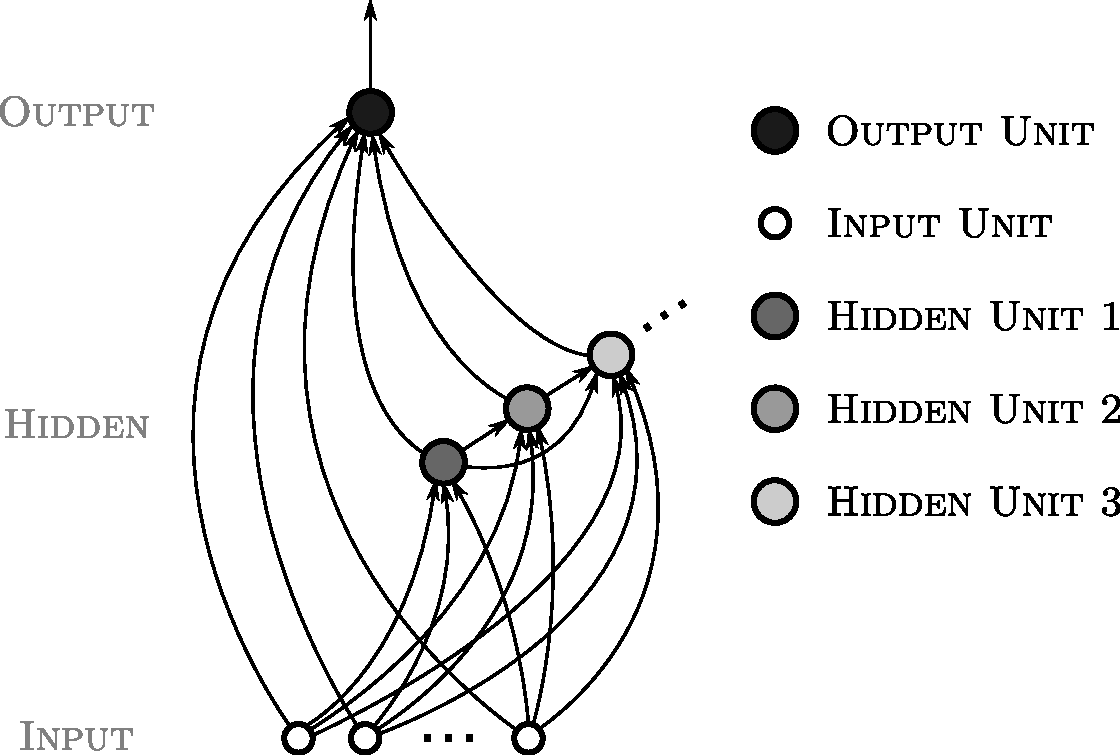
\includegraphics[width=0.6\columnwidth]{img/cascorr}
\medskip
\caption[Cascade Correlation.]{Cascade Correlation. Architettura di una rete con 1 unità di output e 3 unità nascoste.}
\label{fig:intro:cascorr}
\end{figure}

Ad apprendimento ultimato la nuova unità viene stabilmente aggiunta alla rete: i pesi sulle sue connessioni in ingresso vengono ``congelati'', di modo che rimarranno inalterati per il resto del processo di costruzione della rete, ed il suo output viene collegato allo strato di output della rete. Il ``congelamento'' dei pesi sulle connessioni in input alla nuova unità ha risvolti importanti sulle caratteristiche dell'algoritmo. Una volta allenata, infatti, l'unità candidata agirà permanentemente come un \emph{feature detector} e la sua uscita potrà essere presentata allo strato di output o ad altre unità nascoste esattamente come un input aggiuntivo. Benché la rete evolva secondo una architettura a più layer (i.e.\ ogni unità rappresenta un layer a sé stante, figura~\ref{fig:intro:cascorr}), dunque, gli input e le uscite delle unità nascoste possono essere considerati come appartenenti ad un unico strato ai fini dell'allenamento, il che permette l'uso di algoritmi di apprendimento semplici e poco onerosi dal punto di vista computazionale.

Aggiunta una nuova unità nascosta si procede nuovamente con l'allenamento delle connessioni verso l'output della rete, con la valutazione dell'errore commesso ed eventualmente con l'aggiunta di nuove unità, finché il fitting non sia ritenuto soddisfacente. L'algoritmo evolve dunque in maniera \emph{greedy}, aggiungendo unità nascoste finché non siano rispettati determinati criteri di stop.

Per chiarire meglio in che modo evolve la topologia di una rete allenata con Cascade Correlation, la figura~\vref{fig:intro:cascorr} mostra l'architettura di una rete con 3 unità nascoste ed un'unica unità di output.


%%%%%%%%%%%%%%%%%%%%%%%%%%%%%%%%%%%%%%%%%%%%%%%%%%%%%%%%%%%%%%%
%%%%%%%%%%%%%%%%%%%%%%%%%%%%%%%%%%%%%%%%%%%%%%%%%%%%%%%%%%%%%%%
\section{Reti Neurali Ricorrenti}\label{sec:intro:rnn}
Le Reti Neurali Ricorrenti \cite{Tsoi:DiscreteTimeRNN, Haykin:NN} generalizzano le Reti Neurali Feedforward (si veda il paragrafo~\ref{sec:intro:MLeNN}) al trattamento di sequenze. Ciò che distingue le due classi di modelli risiede nel fatto che le Reti Neurali Ricorrenti presentano cicli nella topologia delle connessioni. Questa semplice caratteristica ha un profondo impatto sulle proprietà della rete, in particolare:
\begin{itemize}
\item Per effetto dei cicli nella struttura  delle connessioni, una Rete Neurale Ricorrente può sviluppare e mantenere delle dinamiche interne anche in assenza di input. Reti di questo tipo realizzano infatti un \emph{sistema dinamico}, mentre le Reti Neurali Feedforward realizzano \emph{funzioni}.
\item Se guidate da un segnale di ingresso, le Reti Neurali Ricorrenti mantengono nel proprio stato interno (i.e.\ nelle attivazioni delle proprie unità) una trasformazione non lineare del passato dell'input. La rete possiede dunque una \emph{memoria dinamica} che le permette di elaborare informazioni in un contesto temporale.
\end{itemize}
Grazie all'introduzione di cicli nella topologia, dunque, la rete può essere usata per elaborare dati sequenziali realizzando una \emph{trasduzione di sequenza}, ovvero una funzione da un dominio di sequenze di input ad un dominio di sequenze di output. 

Nella sua forma più semplice una Rete Neurale Ricorrente è composta da un layer di ingresso, un successivo layer nascosto ricorrente (i.e.\ con connessioni cicliche fra le unità) ed un ultimo layer feedforward (i.e.\ con connessioni acicliche) di uscita: il layer nascosto calcola una \emph{funzione locale di encoding} dell'input, mentre il layer di output calcola una \emph{funzione di output}.
Per realizzare l'encoding, in una rete che abbia $N_U$ unità di input ed $N_R$ unità nascoste, il layer nascosto calcola la \emph{funzione di transizione di stato} ricorrente $\tau : \R^{N_U} \times \R^{N_R} \rightarrow \R^{N_R}$ come
\begin{equation}\label{intro:rnn:encoding}
\vect{x}(n) = \tau(\vect{u}(n), \vect{x}(n-1) ) = f( \matr{W}_\textup{in} \vect{u}(n) + \hat{\matr{W}} \vect{x}(n-1) )
\end{equation}
dove $f$ è la funzione di attivazione tipicamente sigmoidale delle unità nascoste, $\vect{u}(n)$ rappresenta l'input $n$-esimo della sequenza, $\vect{x}(t)$ è lo stato interno della rete (i.e.\ le attivazioni delle unità nascoste), la matrice $\matr{W}_\textup{in} \in \R^{N_R \times (N_U + 1)}$ contiene i pesi sulle connessioni dal livello di input al livello nascosto (compreso un \emph{bias}) e la matrice $\hat{\matr{W}} \in \R^{N_R \times N_R}$ contiene i pesi sulle connessioni ricorrenti fra le unità nascoste.\\
Per una rete che abbia $N_Y$ unità di uscita, il layer di output calcola invece la funzione di output $g_\textup{out} : \R^{N_R} \rightarrow \R^{N_Y}$ come
\begin{equation}\label{intro:rnn:output}
\vect{y}(n) = g_\textup{out}(\vect{x}(n)) = f_\textup{out}(\matr{W}_\textup{out} \vect{x}(n))
\end{equation}
dove $\vect{y}(n)$ è l'uscita della rete al passo $n$-esimo, $f_\textup{out}$ è la funzione di attivazione delle unità di output e $\matr{W}_\textup{out} \in \R^{N_Y \times (N_R + 1)}$ contiene i pesi delle connessioni fra il layer nascosto ed il layer di output (più il \emph{bias}).

L'allenamento delle Reti Neurali Ricorrenti usa generalmente tecniche di discesa del gradiente in cui tutte le connessioni della rete vengono modificate per minimizzare l'errore. Gli algoritmi di apprendimento più comuni sono \emph{Back Propagation Through Time} (BPTT) \cite{Werbos:BPTT} e \emph{Real-Time Recurrent Learning} (RTRL) \cite{Williams:RTRL}, che estendono al caso ricorrente le tecniche applicate per l'allenamento di Reti Neurali Feedforward, sfruttando la costruzione di una rete multistrato con topologia aciclica, ottenuta ``copiando'' il layer nascosto, ricorrente, della rete lungo ogni passo della sequenza temporale di input (\emph{unfolding}) \cite{Rumelhart:LearningInternal}.



%%%%%%%%%%%%%%%%%%%%%%%%%%%%%%%%%%%%%%%%%%%%%%%%%%%%%%%%%%%%%%%
%%%%%%%%%%%%%%%%%%%%%%%%%%%%%%%%%%%%%%%%%%%%%%%%%%%%%%%%%%%%%%%

\section{Reservoir Computing}\label{sec:intro:rc}
Il \emph{Reservoir Computing} \cite{Lukosevicius:ESN-Survey,Verstraeten:AnExperimentalUnification,Jaeger:HarnessingNonlinearity} è un paradigma emergente, nell'ambito delle \emph{Reti Neurali Ricorrenti}, che ha origine da due classi di modelli: \emph{Echo State Networks} (ESN) \cite{Jaeger:EchoStateApproach} e \emph{Liquid State Machines} (LSM) \cite{Maas:LSM}.
Benché entrambi i modelli condividano --- e contribuiscano a definire --- i tratti distintivi del Resevoir Computing, nel seguito si farà riferimento in maniera specifica alle ESN, maggiormente legate ad un approccio computazionale\footnote{Le LSM nascono infatti nell'ambito delle neuroscienze e mantengono caratteristiche di forte ispirazione biologica.} e vere progenitrici dei modelli oggetto del lavoro svolto.\\
Prima di descrivere il funzionamento di una ESN, è utile delineare motivazioni, intuizioni e metodi che caratterizzano il Reservoir Computing come paradigma a sé stante per il trattamento di dati strutturati\footnote{Il termine \emph{dati strutturati} è in questo contesto volutamente generico. Benché in questo paragrafo ci si riferisca a dati in forma di sequenze, dominio proprio delle Reti Neurali Ricorrenti e quindi delle ESN, è vero infatti che le caratteristiche del paradigma possono essere riportate a domini strutturati anche più complessi, come i grafi (si veda il paragrafo~\vref{sec:intro:struct:gesn}).}.

Riprendendo quanto descritto nel paragrafo~\ref{sec:intro:rnn}, una generica Rete Neurale Ricorrente viene usata per elaborare dati sequenziali apprendendo una \emph{trasduzione di sequenza}. Tale compito è realizzato modellando un sistema dinamico in cui lo stato interno e l'uscita sono determinati come definito nelle equazioni (\ref{intro:rnn:encoding}) e (\ref{intro:rnn:output}) rispettivamente.
Osservando le formule risulta evidente come l'encoding e l'output giochino un ruolo differente: la \emph{funzione di transizione di stato} $\tau$ implementa infatti un processo di codifica ricorsivo della sequenza in input, che sfrutta informazioni sul contesto ed ha quindi una propria memoria, mentre $\vect{y}(n)$ è il risultato di una funzione pura, senza memoria, della codifica in $\vect{x}(n)$. 

Secondo l'approccio classico, l'allenamento delle Reti Neurali Ricorrenti usa tecniche di discesa del gradiente che prevedono l'adattamento di tutti i pesi della rete: nessuna suddivisione concettuale fra stato interno ed output viene realizzata benché le differenze emergano dal punto di vista algoritmico (l'output, a differenza dello stato interno, è infatti direttamente confrontabile con il target). Gli algoritmi di apprendimento più comuni, \emph{Back Propagation Through Time} (BPTT) \cite{Werbos:BPTT} e \emph{Real-Time Recurrent Learning} (RTRL) \cite{Williams:RTRL}, soffrono tuttavia di alcuni svantaggi. In particolare:
\begin{itemize}
\item L'aggiornamento graduale dei parametri può modificare le dinamiche della rete fino a far degenerare le informazioni del gradiente, di modo che la convergenza possa non essere garantita \cite{Doya:Bifurcations}.
\item Il costo computazionale per l'aggiornamento è molto alto ---  $O(N^2)$ per BPTT e $O(N^4)$ per RTRL, in una rete con $N$ unità --- e riduce la possibilità di utilizzare reti di grandi dimensioni.
\item Il gradiente decresce esponenzialmente nel tempo, per cui risulta difficile apprendere dipendenze a lungo termine \cite{Bengio:TheProblemOfLearning}.
\end{itemize}

Il paradigma del Reservoir Computing nasce dunque con l'idea di evitare almeno parzialmente questi problemi adottando un approccio radicalmente differente:
\begin{itemize}
\item Una rete neurale ricorrente, chiamata \emph{reservoir}, viene generata \emph{in maniera casuale} ed ha lo scopo di espandere il segnale in input, mantenendo nel proprio stato interno una trasformazione non lineare del passato. I pesi del reservoir rimangono \emph{inalterati} durante il training. 
\item L'output viene generato come una \emph{combinazione lineare} dei segnali provenienti dalle unità del reservoir, passivamente eccitate dall'input. Il \emph{readout} lineare viene adattato, in fase di learning, utilizzando il segnale del teacher come target.
\end{itemize}
La suddivisione fra stato interno della rete ed output è quindi in questo caso resa esplicita e si sfrutta la capacità del reservoir di mantenere una trasformazione non lineare del passato, anche senza dover effettuare l'apprendimento \cite{Tino:MarkovianArchitecturalBias}, per limitare l'azione del learning al solo readout.

Benché il Reservoir Computing si caratterizzi come un paradigma a sé, è giusto osservare che l'idea di gestire in maniera specifica e separata readout e stato interno trova altri esempi nell'ambito del Machine Learning: è il caso, ad esempio, dell'algoritmo di apprendimento \emph{Backpropagation-Decorrelation}\footnote{Per le sue caratteristiche, l'algoritmo BPDC viene talvolta indicato a tutti gli effetti come appartenente all'ambito del Reservoir Computing. Si veda, ad esempio, \cite{Song:Effects}.} (BPDC) \cite{Steil:BPDC} o delle \emph{Extreme Learning Machines} (ELM) \cite{Huang:ELM}. In termini ancor più generali, l'approccio del Reservoir Computing è inoltre riconducibile all'utilizzo di un kernel, come sottolineato anche in \cite{Jaeger:SpecialIssue}. 


%%%%%%%%%%%%%%%%%%%%%%%%%%%%%%%%%%%%%%%%%%%%%%%%%%%%%%%%%%%%%%%
\subsection{Echo State Networks}\label{sec:intro:rc:esn}
Definiamo formalmente le ESN \cite{Jaeger:EchoStateApproach, Jaeger:ShortTermMemory, Jaeger:HarnessingNonlinearity}, fissando anche parte della terminologia che verrà adottata nel seguito.

Consideriamo una rete con $N_U$ unità di input, $N_R$ unità ricorrenti interne (reservoir), ed $N_Y$ unità di output. 
Indichiamo con $\vect{u}(n) \in \R^{N_U}$ l'input all'istante $n$, appartenente alla sequenza $s(\vect{u}) = [\vect{u}(1), \vect{u}(2), \dots, \vect{u}(k)]$, con $\vect{x}(n) \in \R^{N_R}$ le attivazioni delle unità del reservoir e con $\vect{y}(n) \in \R^{N_Y}$ l'output.\\
Usiamo le seguenti matrici per i pesi delle connessioni: $\matr{W}_\textup{in} \in \R^{N_R \times (N_U+1)}$ per l'input, $\matr{W} \in \R^{N_R \times N_R}$ per le connessioni interne e $\matr{W}_\textup{out} \in \R^{N_Y \times (N_R+1)}$ per le connessioni verso le unità di output, ovvero verso il readout.\\
Le equazioni di base che determinano l'evoluzione del sistema sono le seguenti:
\begin{equation}\label{eq:intro:esn}
\begin{array}{l}
\vect{x}(n) = \tau( \vect{u}(n), \vect{x}(n-1) ) = f( \matr{W}_{\textup{in}} \vect{u}(n) + \hat{\matr{W}} \vect{x}(n-1) ) \\
\vect{y}(n) = g_\textup{out}( \vect{x}(n) ) = f_{\textup{out}}( \matr{W}_{\textup{out}} \vect{x}(n) )
\end{array}
\end{equation}
dove $f$ ed $f_{\textup{out}}$ sono funzioni applicate elemento per elemento e corrispondono rispettivamente alle funzioni di attivazione delle unità del reservoir, tipicamente sigmoidali (e.g.\ $\tanh$), e delle unità di output, tipicamente lineari.
La figura~\ref{fig:intro:esn} mostra in maniera schematica la struttura di una ESN come quella descritta dall'equazione (\ref{eq:intro:esn}).

\begin{figure}[tbp]
\centering
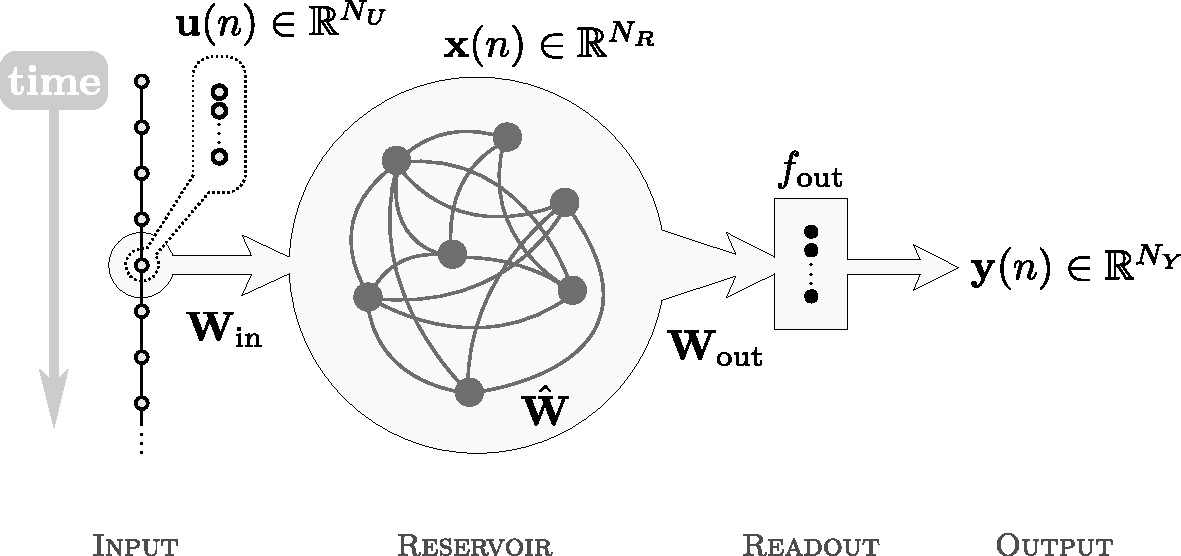
\includegraphics[width=0.8\columnwidth]{img/ESN}
\medskip
\caption[Echo State Network.]{Schematizzazione grafica di una Echo State Network (ESN).}
\label{fig:intro:esn}
\end{figure}

Varianti comuni all'equazione (\ref{eq:intro:esn}) prevedono inoltre l'esistenza di connessioni dirette dall'input al readout o all'indietro, dal readout al reservoir (si veda ad esempio \cite{Jaeger:EchoStateApproach, Jaeger:ShortTermMemory}). La presenza di queste ultime in particolare implica considerazioni specifiche e risulta interessante ai fini del lavoro svolto. L'introduzione di connessioni che portino informazione all'interno del reservoir risponde infatti ad un limite specifico del Reservoir Computing: la presenza di dinamiche fissate a priori, che non vengono adattate sulla base del task affrontato. Con l'introduzione di connessioni all'indietro, dal readout verso il reservoir, si cerca dunque di realizzare un meccanismo, che chiameremo di \emph{output-feedback}, che permetta di influenzare le dinamiche del reservoir in maniera consistente con il problema che si vuole risolvere. Una soluzione di questo tipo presenta tuttavia dei problemi. In particolare:
\begin{itemize}
\item La presenza di di connessioni all'indietro, dal readout al reservoir, tende a determinare situazioni di instabilità nel modello \cite{Lukosevicius:ESNwithTrainedFeedbacks, Wyffels:stableOutputFeedback}, e risulta dunque di difficile applicazione.
\item Il sistema di output-feedback proposto per le ESN non risulta direttamente generalizzabile al caso in cui si trattino domini di input più complessi delle sequenze (si veda il paragrafo~\vref{sec:intro:struct:gesn}).
\item La presenza di output-feedback, può avere l'effetto di influenzare le dinamiche del reservoir, ma non quello di introdurvi effettivamente informazione supervisionata. Al passo $n$, infatti, il segnale di output-feedback introduce nel reservoir un segnale corrispondente all'uscita della rete al passo $n-1$, che non ha legami con l'uscita desiderata al passo $n$-esimo. 
\end{itemize}
Per questi motivi, l'introduzione di un meccanismo stabile di output-feedback è ad oggi un tema aperto nell'ambito del Reservoir Computing.

L'allenamento di una ESN avviene, in maniera supervisionata, sulla base dei valori target $\vect{y}_{\textup{target}}(n)$. A differenza di quanto accade nell'approccio classico, solo $\matr{W}_{\textup{out}}$ è interessata dall'aggiornamento dei pesi in fase di learning, mentre le altre matrici dei pesi rimangono invariate. Proprio per questa caratteristica è tuttavia necessario che le matrici $\matr{W}_{\textup{in}}$ e $\hat{\matr{W}}$ soddisfino determinati requisiti: informalmente possiamo dire che è necessario che lo stato interno della rete sia un'\emph{eco} della sequenza in input.

In \cite{Jaeger:EchoStateApproach, Jaeger:ShortTermMemory} viene definita la \emph{echo state property}, che descrive la condizione basilare per il corretto funzionamento del reservoir. Intuitivamente la echo state property implica che l'effetto dello stato $\vect{x}(n)$ e dell'input $\vect{u}(n)$ sugli stati futuri, $\vect{x}(n+t)$, svanisca con il passare del tempo ($t \rightarrow \infty$), senza persistere né essere amplificato. Di conseguenza le attivazioni della rete, dopo una fase transitoria, dipenderanno unicamente dalla sequenza in input e non dallo stato iniziale, che può dunque essere arbitrario. 

Assumendo che una rete abbia funzioni di attivazione sigmoidali è possibile individuare una condizione sufficiente per il verificarsi di una simile situazione ed una condizione sufficiente perché invece non si verifichi. Sia la matrice $\hat{\matr{W}}$ tale che 
\begin{equation}
\sigma_{max} < 1
\end{equation}
con $\sigma_{max}$ massimo valore singolare, allora la rete possiede la echo state property per ogni input ammissibile $s(\vect{u})$.\\
Sia la matrice $\hat{\matr{W}}$ tale da avere raggio spettrale 
\begin{equation}
\rho(\hat{\matr{W}}) = \abs{\lambda_{max}} > 1
\end{equation}
dove $\lambda_{max}$ è l'autovalore di modulo massimo, allora la rete non ha la echo state property se la sequenza nulla è un input ammissibile. 

In \cite{Gallicchio:ArchitecturalAndMarkovian} la presenza della echo state property viene messa in relazione con la \emph{contrattività} della funzione di transizione di stato $\tau$. In particolare si dimostra che se $\tau$ è contrattiva con parametro $C < 1$, ovvero
\begin{multline}
\exists C \in [0,1) \mbox{ tale che } \forall \vect{u} \in \R^{N_U}, \forall \vect{x}, \vect{x}' \in \R^{N_R} : \\
\vectnorm{\tau(\vect{u}, \vect{x}) - \tau(\vect{u}, \vect{x}')} \leq C \vectnorm{\vect{x} - \vect{x}'}
\end{multline}
per una qualsiasi norma $\vectnorm{\cdot}$ nello spazio degli stati $\R^{N_R}$, allora la echo state property è garantita. Oltre ad assicurare la stabilità della rete, la contrattività della funzione di transizione di stato del reservoir determina dei vincoli sull'evoluzione degli stati della rete. Lo spazio degli stati del reservoir risulta infatti avere una \emph{natura Markoviana}: gli stati corrispondenti a due diverse sequenze di input che abbiano un suffisso comune saranno tanto più vicini quanto maggiore sarà la lunghezza del suffisso comune. Questo cosiddetto bias Markoviano ha forte influenza sulla capacità computazionale del modello: in \cite{Hammer:RNNWithSmallWeights, Tino:MarkovianArchitecturalBias} si mostra come una Rete Neurale Ricorrente che abbia una funzione di transizione di stato contrattiva e spazio degli stati limitato possa essere approssimata arbitrariamente bene dalla classe dei modelli su sequenze con dinamiche di stato Markoviane (e.g.\ Variable Memory Length Markov Models \cite{Ron:ThePowerOfAmnesia}). Ne risulta che, anche senza alcun learning, gli stati interni corrispondenti a sequenze di input con suffissi comuni tendano ad essere naturalmente raggruppati o, in altri termini, che la rete abbia per una propria caratteristica architetturale la capacità di discriminare le sequenze di input sulla base del loro suffisso.\\
Questo bias architetturale Markoviano, come visto strettamente legato alla echo state property, rappresenta di fatto l'essenza del modello e ne giustifica l'intuizione di base: sfruttare le caratteristiche strutturali del reservoir per realizzare un processo di encoding in grado di discriminare sequenze con suffissi diversi anche in assenza di un processo specifico di adattamento, per limitare l'azione del learning alla sola, semplice, funzione di output $g_\textup{out}$. 
Di contro, secondo una visione complementare, il vantaggio computazionale è ottenuto nelle ESN accettando la presenza di dinamiche definite a priori, che non vengono adattate per risolvere il task specifico affrontato e che limitano dunque la capacità espressiva del modello.

%sfruttare le caratteristiche strutturali della rete, in grado di per sé di discriminare sequenze con suffissi diversi, per limitare l'azione del learning alla sola, semplice, funzione di output $g_\textup{out}$. 


Nonostante l'apprendimento richieda un basso costo in termini computazionali, le ESN sono state applicate con successo a molti problemi ottenendo risultati migliori rispetto ad altri approcci precedenti (si veda ad esempio \cite{Jaeger:HarnessingNonlinearity}, \cite[pag.~8]{Schrauwen:AnOverview}, o \cite[pag.~5]{Lukosevicius:ESN-Survey} per un elenco dettagliato). Il modello è inoltre semplice e segue un paradigma molto generale: questo offre ampi margini di scelta e sperimentazione nell'implementazione del learning, nella topologia, nella scelta delle funzioni utilizzate e addirittura nell'implementazione fisica della rete\footnote{Si veda \cite{Fernando:PatternRecognition} per un esempio in cui la rete --- basata però su LSM --- viene implementata attraverso hardware ``poco convenzionale''.}. Fra gli aspetti positivi delle ESN è infine opportuno menzionare l'alta plausibilità biologica, che caratterizza il Reservoir Computing in generale e che continua a rappresentare un fattore importante nell'ambito delle Reti Neurali.

Le ESN mostrano tuttavia anche dei limiti: alcuni di natura intrinseca al modello, come l'alto numero di unità impiegate che rende difficile l'implementazione fisica con risorse hardware limitate \cite{Prokhorov:AppealAndChallenges}, ed altri legati al fatto che la ricerca in materia sia ancora in una fase poco avanzata. Gli effetti del rumore nei dati in input o la replicabilità delle condizioni di buon funzionamento della rete sono ad esempio fattori determinanti ma non completamente spiegati, che possono mettere in dubbio l'applicabilità del modello ad ampie classi di problemi \cite{Prokhorov:AppealAndChallenges}.

Per contestualizzare meglio quanto verrà descritto in seguito è inoltre opportuno sottolineare come la ricerca sulle ESN sia ad oggi in larghissima parte orientata all'apprendimento di trasduzioni di sequenze e come l'applicazione dei principi del Reservoir Computing nell'ambito del trattamento di domini più complessi, come alberi o grafi, sia da considerarsi di vivissima attualità.



%%%%%%%%%%%%%%%%%%%%%%%%%%%%%%%%%%%%%%%%%%%%%%%%%%%%%%%%%%%%%%%
%%%%%%%%%%%%%%%%%%%%%%%%%%%%%%%%%%%%%%%%%%%%%%%%%%%%%%%%%%%%%%%

\section{Modelli per domini strutturati}\label{sec:intro:struct}
La possibilità di trattare domini di input in cui le informazioni siano strutturate (e.g.\ grafi) rappresenta una delle sfide che attualmente dominano e danno impulso ad una parte del mondo del Machine Learning. Molti problemi dell'informatica, della chimica, relativi all'elaborazione del linguaggio naturale, all'analisi di immagini o documenti, trovano infatti una propria naturale formulazione all'interno di domini più complessi della semplice rappresentazione tramite vettori numerici o sequenze. 

Nell'ambito neurale, le \emph{Reti Neurali Ricorsive} \cite{Frasconi:AGeneralFramework, Sperduti:SupervisedNeuralNetworks} generalizzano le Reti Neurali Ricorrenti (si veda il paragrafo~\ref{sec:intro:rnn}) affinché possano gestire domini di input strutturati. Reti di questo tipo sono basate su un processo di encoding in cui gli stati vengono calcolati ricorsivamente in accordo con le relazioni topologiche fra i vertici dell'input. La possibilità di tenere in considerazione la topologia durante l'encoding e di far sì che l'intero processo sia adattivo, delimita la separazione, sia concettuale che pratica, tra le Reti Neurali Ricorsive e l'approccio classico, che prevede invece l'uso di conoscenza pregressa per codificare i dati (e.g.\ estraendo indici topologici \cite{Hall:TheMolecularConnectivity}).

Il processo di encoding rappresenta dunque la chiave dell'approccio che caratterizza i modelli neurali ricorsivi: ne determina i vantaggi e, tuttavia, ne mette anche in luce i limiti. In particolare, per garantire che ogni input abbia una rappresentazione appropriata, ovvero per evitare condizioni cicliche nel processo di encoding, si ricorre all'assunzione di \emph{causalità} del sistema di transizione \cite{Sperduti:SupervisedNeuralNetworks}. Essendo la codifica ``guidata'' dalla topologia dell'input, si assume infatti che lo stato corrispondente ad un vertice dipenda unicamente dall'etichetta del vertice stesso e dagli stati corrispondenti ai vertici discendenti da esso. Se questo ha il vantaggio di garantire la convergenza ha, d'altra parte, forte impatto sulla classe degli input trattabili: l'assunzione di causalità impone infatti la presenza di un ordinamento topologico fra i vertici, limitando il dominio di input alla classe dei Grafi Diretti Aciclici (che comprende gli alberi radicati).

Nella storia recente delle Reti Neurali Ricorsive si ritrovano tuttavia dei modelli tesi a superare le limitazioni imposte dal vincolo di causalità. Ai fini di una completa comprensione del lavoro svolto, siamo particolarmente interessati a menzionare due approcci che, seppur non direttamente legati fra loro, trovano una sintesi nei modelli proposti.

Prima con la \emph{Contextual Recursive Cascade Correlation} (CRCC) \cite{Micheli:ContextualProcessing, Hammer:UniversalApproximation} poi con il modello \emph{Neural Network for Graphs} (NN4G) \cite{Micheli:NN4G}, si fa leva sull'approccio costruttivo per limitare e poi superare gli effetti dell'assunzione di causalità. In particolare NN4G sfrutta il processo incrementale di costruzione della rete per comporre una rete feedforward, che non risenta dunque delle eventuali dipendenze cicliche nell'input. I modelli citati mettono anche l'accento sull'importanza del fatto che, durante il processo di costruzione della rete, le nuove unità possano usufruire delle informazioni rese disponibili dalle unità precedenti (i.e.\ le unità ``congelate''). Questa caratteristica, vera anche nel caso delle reti feedforward, acquisisce particolare rilevanza nel caso di input strutturati: lo stato di ogni unità è infatti funzione anche della topologia dell'input. Per questo le informazioni trasmesse alle unità successive contribuisco alla formazione di un \emph{contesto}, che cresce con il crescere della rete \cite{Micheli:NN4G}. L'approccio costruttivo permette dunque a questi modelli di sfruttare informazioni contestuali altrimenti inaccessibili.

Un secondo approccio per garantire la stabilità del processo di encoding anche in presenza di dipendenze cicliche nell'input fa invece affidamento su un setting contrattivo della funzione di transizione di stato (si veda il paragrafo~\ref{sec:intro:rc:esn}). Rientrano in questo filone i modelli \emph{Graph Neural Network} (GNN) \cite{Scarselli:GNN} e le \emph{Graph Echo State Network} (GraphESN). 
Mentre in GNN la contrattività è il risultato di un processo iterativo di apprendimento, che coinvolge tutti i pesi della rete, le GraphESN ricorrono alla contrattività della funzione di transizione di stato in accordo ai principi del Reservoir Computing, sfruttando dunque la presenza di un reservoir fisso e di un readout adattivo.
In quanto diretta progenitrice dei modelli proposti, quest'ultima tipologia di reti verrà discussa in dettaglio nel seguito (si veda il paragrafo~\ref{sec:intro:struct:gesn}), non prima di aver introdotto formalmente il problema dell'apprendimento su domini strutturati.


%%%%%%%%%%%%%%%%%%%%%%%%%%%%%%%%%%%%%%%%%%%%%%%%%%%%%%%%%%%%%%%%%%%
\subsection{Trasduzioni su domini strutturati}\label{sec:intro:struct:terminologia}
Nel corso di questo paragrafo sarà formulato il problema dell'apprendimento su domini strutturati, introducendo terminologia e notazione che verranno utilizzate nel corso della tesi.

Un grafo $\graph{g}$, appartenente ad un insieme di grafi $\mathcal{G}$, è una coppia $(V(\graph{g}), E(\graph{g}))$, dove $V(\graph{g})$ denota l'insieme dei vertici di $\graph{g}$ ed $E(\graph{g}) = \setdef{(u,v)}{u, v \in V(\graph{g})}$ denota l'insieme di archi di $\graph{g}$. Per semplicità nel seguito gli insiemi $V(\graph{g})$ e $E(\graph{g})$ saranno talvolta indicati come $V$ ed $E$ rispettivamente, mantenendo implicito il riferimento al grafo $\graph{g}$. Nel caso di grafi indiretti definiamo i \emph{vicini} del vertice $v$ di un grafo come l'insieme dei vertici ad esso adiacenti\footnote{Nel caso di grafi diretti è possibile un'ulteriore suddivisione dei vertici adiacenti in \emph{predecessori} e \emph{successori}. Per semplicità e per una maggiore aderenza ai task affrontati questa formulazione viene tralasciata.}, $\mathcal{N}(v) = \setdef{u \in V}{(u,v) \in E}$. Sia il grado di un vertice $v$ il numero dei suoi vicini, $degree(v) = \abs{\mathcal{N}(v)}$, indichiamo con $k$ il \emph{grado massimo} riscontrabile sull'insieme $\mathcal{G}$.
Diciamo che due grafi $\graph{g}_1 = (V(\graph{g}_1), E(\graph{g_1}))$ e $\graph{g}_2 = (V(\graph{g}_2), E(\graph{g_2}))$ sono \emph{isomorfi} se esiste una funzione bigettiva $f : V(\graph{g}_1) \rightarrow V(\graph{g}_2)$ tale che $(u,v) \in E(\graph{g_1})$ se e solo se $(f(u), f(v)) \in E(\graph{g_2})$ (si veda anche \cite{Hammer:AdaptiveContextualProcessing}). 

Consideriamo che ad ogni vertice di un grafo sia associata un'etichetta numerica $\vect{u}(v) \in \R^{N_U}$, dove $\R^{N_U}$ denota uno spazio di input di etichette vettoriali. Indichiamo l'insieme dei grafi con etichette in $\R^{N_U}$ con $(\R^{N_U})^{\#}$.

Obiettivo di un modello per domini strutturati è l'apprendimento di una \emph{trasduzione strutturale} $\mathcal{T}$, ovvero di una funzione da un dominio di grafi in input $(\R^{N_U})^{\#}$ ad un dominio di grafi in output $(\R^{N_Y})^{\#}$:
\begin{equation}\label{eq:transduction}
\mathcal{T} : (\R^{N_U})^{\#} \rightarrow (\R^{N_Y})^{\#}
\end{equation}
Indichiamo con $\vect{y}(v) \in \R^{N_Y}$ l'etichetta vettoriale associata al vertice $v$ del grafo nel dominio di output. 

Distinguiamo due tipi di trasduzioni. In una trasduzione \emph{structure-to-structure} (anche chiamata \emph{node-focused} \cite{Scarselli:GNN}) il grafo in output è isomorfo a quello in input, ovvero $\mathcal{T}$ associa un vertice in output ad ogni vertice dell'input, mantenendone inalterata la struttura. In una trasduzione \emph{structure-to-element} (o \emph{graph-focused} \cite{Scarselli:GNN}), invece, un singolo output vettoriale, $\vect{y}(\graph{g}) \in \R^{N_Y}$, è associato all'intero grafo. La figura~\ref{fig:intro:trasduzione-s2s} e la figura~\ref{fig:intro:trasduzione-s2e} mostrano schematicamente i due tipi di trasduzione strutturale descritti.

\begin{figure}[tbp]
\centering
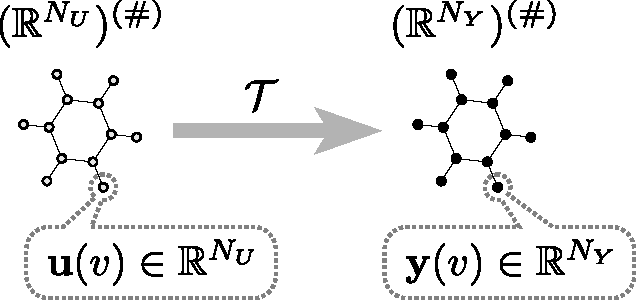
\includegraphics[width=0.5\columnwidth]{img/T-str2str}
\medskip
\caption{Trasduzione structure-to-structure.}
\label{fig:intro:trasduzione-s2s}
\end{figure}

\begin{figure}[tbp]
\centering
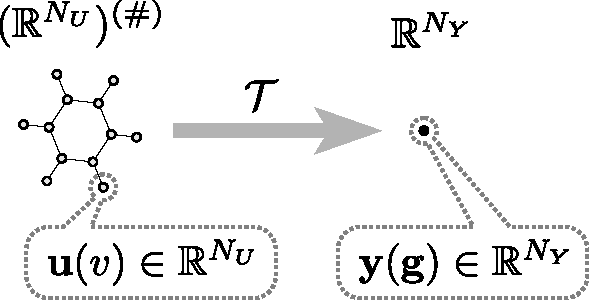
\includegraphics[width=0.5\columnwidth]{img/T-str2el}
\medskip
\caption{Trasduzione structure-to-element.}
\label{fig:intro:trasduzione-s2e}
\end{figure}

Nel caso dell'apprendimento supervisionato, l'allenamento avviene avvalendosi di un training-set $\mathfrak{T} = \setdef{(\graph{g}, \vect{y}_\textup{target}(g))}{\graph{g} \in \mathcal{G}, \vect{y}_\textup{target}(\graph{g}) \in (\R^{N_Y})^{\#}}$, dove $\vect{y}_\textup{target}(\graph{g})$ indica il target associato ad uno specifico input e può essere un grafo etichettato (isomorfo a $\graph{g}$) nel caso di trasduzioni structure-to-structure o un vettore di reali a dimensione fissa nel caso di trasduzioni structure-to-element.


%%%%%%%%%%%%%%%%%%%%%%%%%%%%%%%%%%%%%%%%%%%%%%%%%%%%%%%%%%%%%%%%%%%
\subsection{Graph Echo State Networks}\label{sec:intro:struct:gesn}
Le \emph{Graph Echo State Network} (GraphESN) \cite{Gallicchio:GraphESN} rappresentano un'estensione delle ESN (si veda il paragrafo~\ref{sec:intro:rc:esn}) --- e delle TreeESN \cite{Gallicchio:TreeESN} --- per il trattamento del dominio dei grafi.

In maniera simile ad una ESN, in una GraphESN sono distinguibili tre layer: uno di \emph{input}, uno nascosto detto \emph{reservoir} e formato da unità ricorsive e non lineari ed infine un \emph{readout} feedforward. Anche in questo caso è richiesto che la funzione di transizione di stato del reservoir sia contrattiva. Il reservoir viene dunque inizializzato affinché rispetti tale vincolo e rimane poi inalterato, mentre il solo readout viene allenato.\\
\`E importante sottolineare come la contrattività della funzione di transizione di stato assuma in questo caso un significato specifico di grossa rilevanza, ampliando la classe delle strutture supportate dal modello. La contrattività garantisce infatti la stabilità del processo di codifica anche nel caso di dipendenze cicliche fra le variabili di stato (si veda il paragrafo~\ref{sec:intro:struct}), determinando l'applicabilità del modello ad una classe di strutture che comprende grafi non diretti e/o ciclici.

Passiamo ora a caratterizzare più formalmente una GraphESN come modello per l'apprendimento di trasduzioni strutturali su un dominio di grafi.

Riprendendo quanto descritto in precedenza (si veda il paragrafo~\ref{sec:intro:struct:terminologia}), una trasduzione strutturale (\ref{eq:transduction}) può essere efficacemente decomposta come 
\begin{equation}\label{eq:intro:gesn:trasd}
\mathcal{T} = \mathcal{T}_\textup{out} \circ \mathcal{T}_\textup{enc}
\end{equation} 
dove $\mathcal{T}_\textup{enc} : (\R^{N_U})^{\#} \rightarrow (\R^{N_R})^{\#}$ è una \emph{funzione di encoding}, che mappa l'input in un dominio strutturato di features, e $\mathcal{T}_\textup{out} : (\R^{N_R})^{\#} \rightarrow (\R^{N_Y})^{\#}$ la \emph{funzione di output}. 
La figura~\ref{fig:intro:T-enc-out} mostra la realizzazione di una generica trasduzione strutturale (structure-to-structure) attraverso la composizione di una funzione di encoding, $\mathcal{T}_\textup{enc}$, ed una funzione di output, $\mathcal{T}_\textup{out}$.
\begin{figure}[tbp]
\centering
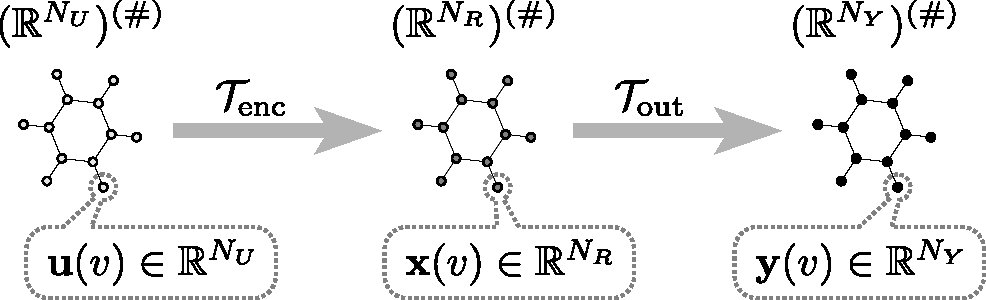
\includegraphics[width=0.8\columnwidth]{img/T-enc-out}
\medskip
\caption[Decomposizione di una trasduzione strutturale.]{Decomposizione di una trasduzione strutturale tramite una funzione di encoding $\mathcal{T}_\textup{enc}$ ed una funzione di output $\mathcal{T}_\textup{out}$.}
\label{fig:intro:T-enc-out}
\end{figure}

Secondo l'approccio neurale --- ricorsivo e ricorrente --- la funzione di encoding $\mathcal{T}_\textup{enc}$ viene realizzata da un sistema dinamico; lo spazio delle features $(\R^{N_R})^{\#}$ è composto da variabili di stato, associate ad ogni vertice dell'input. Chiamiamo $\vect{x}(v) \in \R^{N_R}$ l'informazione di stato associata al vertice $v$ del grafo in input $\graph{g}$. Indichiamo inoltre con $\vect{x}(\graph{g}) \in \R^{\abs{V(\graph{g})} N_R}$ la concatenazione degli stati associati a tutti i vertici dell'input, secondo un ordine arbitrario, e con $\vect{x}(\mathcal{N}(v)) \in \R^{\abs{\mathcal{N}(v)} N_R}$ la concatenazione degli stati associati ai vicini di un vertice $v$. La funzione $\mathcal{T}_\textup{enc}$ associa dunque ad ogni vertice dell'input $v \in V(\graph{g})$ una corrispondente informazione di stato secondo una \emph{funzione locale di encoding} $\tau$
\begin{equation}\label{eq:localenc}
\vect{x}(v) = \tau(\vect{u}(v), \mathcal{N}(v))
\end{equation}
che esprime la dipendenza dello stato associato al vertice $v$ da quelli associati ai suoi vicini. Equivalentemente possiamo dire che l'applicazione dell'equazione (\ref{eq:localenc}) ad ogni vertice dell'input realizza la \emph{funzione globale di encoding} $\hat{\tau}$
\begin{equation}\label{eq:globalenc}
\vect{x}(\graph{g}) = \hat{\tau}(\graph{g}, \vect{x}(\graph{g}))
\end{equation}
Dato un grafo in input $\graph{g}$, dunque, l'output della funzione di encoding $\mathcal{T}_\textup{enc}$ corrisponde alla soluzione dell'equazione (\ref{eq:globalenc}).

In una GraphESN la funzione $\mathcal{T}_\textup{enc}$ viene realizzata dal reservoir, che calcola iterativamente una \emph{funzione di transizione locale di stato}, versione iterativa dell'equazione (\ref{eq:localenc}). Al passo $t$, la funzione associa ad ogni vertice $v$ una codifica, o valore di stato, $\vect{x}_t(v)$ secondo la seguente equazione
\begin{equation}\label{intro:gesn:reservoir}
\vect{x}_t(v) 	= \tau( \vect{u}(v), \vect{x}_{t-1}(\mathcal{N}(v)) ) 
				= f( \matr{W}_{\textup{in}} \vect{u}(n) + \sum_{w \in \mathcal{N}(v)} \hat{\matr{W}} \vect{x}_{t-1}(w) )
\end{equation}
dove $\matr{W}_{\textup{in}} \in \R^{N_R \times (N_U + 1)}$ è la matrice dei pesi sulle connessioni tra input e reservoir, $\hat{\matr{W}} \in \R^{N_R \times N_R}$ è la matrice dei pesi ricorrenti tra i vicini di un vertice ed $f$ è la funzione di attivazione, tipicamente sigmoidale, delle unità del reservoir. La figura~\vref{fig:intro:encoding-step} mostra un passo del procedimento iterativo di encoding, evidenziando come lo stato calcolato per ogni vertice $v$ dipenda dall'etichetta numerica di input corrispondente, $\vect{u}(v)$, nonché dallo stato in corrispondenza dei vertici vicini calcolato al passo precedente, $\vect{x}(\mathcal{N}(v))$.

\begin{figure}[tbp]
\centering
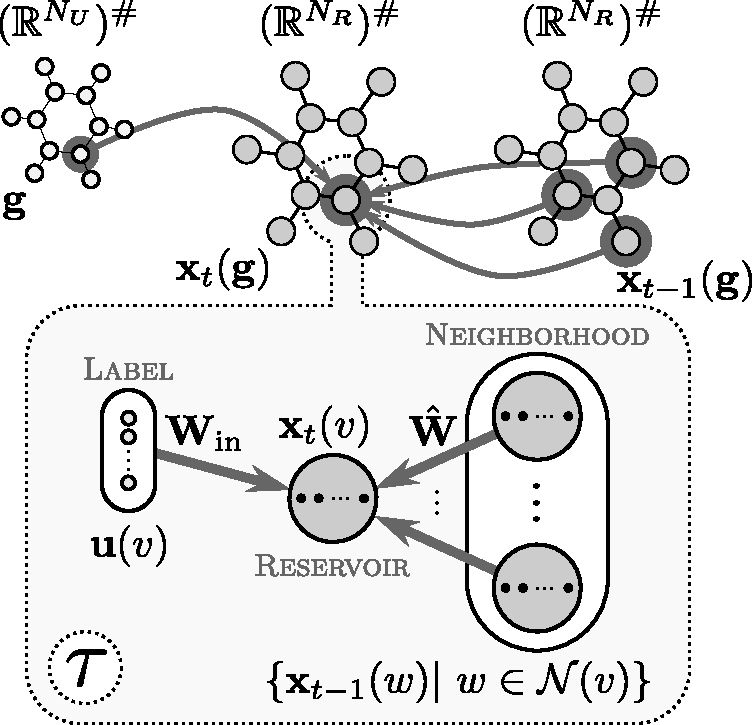
\includegraphics[width=0.6\columnwidth]{img/GraphESN-reservoir-application}
\medskip
\caption[Funzione di transizione locale di stato]{Schema di applicazione della funzione di transizione locale di stato ad un vertice $v$ dell'input $\graph{g}$.}
\label{fig:intro:encoding-step}
\end{figure}

Per poter garantire che l'encoding converga, e quindi che l'equazione (\ref{eq:globalenc}) abbia una soluzione, si ricorre ad un setting contrattivo della funzione $\tau$. Perché $\tau$ sia \emph{contrattiva} rispetto allo stato, è necessario che valga la seguente condizione:
\begin{multline}
\exists C \in [0,1) \mbox{ tale che } \forall \vect{u} \in \R^{N_U}, \forall \vect{x}_1, \dots , \vect{x}_k, \vect{x}'_1, \dots , \vect{x}'_k \in \R^{N_R} : \\
\vectnorm{\tau(\vect{u}, \vect{x}_1, \dots , \vect{x}_k) - \tau(\vect{u}, \vect{x}'_1, \dots , \vect{x}'_k)} \leq C \max_{i = 1, \dots ,k} \vectnorm{\vect{x}_i - \vect{x}'_i}
\end{multline}
dove $\vectnorm{\cdot}$ è una qualsiasi norma su $\R^{N_R}$. Considerando per $\tau$ l'implementazione dell'equazione~(\ref{intro:gesn:reservoir}), con $f=\tanh$ usata come funzione di attivazione delle unità del reservoir, e scegliendo la distanza euclidea come norma, risulta che la contrattività è garantita per \cite{Gallicchio:ExploitingVerticesStates}
\begin{equation}\label{eq:intro:gesn:sigma}
\sigma = \vectnorm{\hat{\matr{W}}}_2 k < 1
\end{equation}
dove $k$ è il grado massimo calcolato su tutti i grafi in $\mathcal{G}$ e $\sigma$, che controlla il grado di contrattività delle dinamiche del reservoir, è chiamato \emph{coefficiente di contrazione}. Una volta che la contrattività di $\tau$ sia assicurata, la convergenza del calcolo iterativo del reservoir è garantita dal \emph{Principio di Contrazione di Banach} \cite{Martelli:IntroductionToDiscrete} per ogni stato iniziale $\vect{x}_0(\graph{g})$; nella pratica questo permette di calcolare la codifica di un grafo in maniera iterativa, interrompendo l'elaborazione una volta che, per ogni vertice del grafo, la distanza tra due stati successivi nel processo di encoding sia inferiore ad una soglia prefissata $\epsilon$: $\vectnorm{\vect{x}_t(v) - \vect{x}_{t-1}(v)}_2 \leq \epsilon$. L'algoritmo~\vref{alg:intro:gesn:reservoir} mostra il processo di codifica ricorsivo implementato dal reservoir di una GraphESN.

\begin{algorithm}[tb]
\caption{GraphESN: algoritmo iterativo di encoding.}
\label{alg:intro:gesn:reservoir}
\begin{algorithmic}
\FORALL{$\graph{g} \in \mathcal{G}$}
	\STATE $t = 0$
	\FORALL{$v \in V(\graph{g})$}
		\STATE $\vect{x}_0(v) = 0$
	\ENDFOR
	\REPEAT
		\STATE $t = t+1$
		\FORALL{$v \in V(\graph{g})$}
			\STATE $\vect{x}_t(v) = \tau(\vect{u}(v), \vect{x}_{t-1}(\mathcal{N}(v)))$
		\ENDFOR
	\UNTIL{$\forall v \in V(\graph{g}) : \vectnorm{\vect{x}_t(v) - \vect{x}_{t-1}(v)}_2 \leq \epsilon$}
\ENDFOR
\RETURN $\vect{x}(\graph{g})$
\end{algorithmic}
\end{algorithm}

\`E opportuno sottolineare come la contrattività della funzione di transizione di stato caratterizza le GraphESN sotto diversi importanti aspetti, che vanno oltre quello algoritmico. Innanzi tutto la stabilità del processo di codifica rende le GraphESN in grado di gestire grafi ciclici, il che rappresenta invece un problema per le reti ricorrenti classiche. Inoltre la contrattività implica la echo state property (si veda il paragrafo~\ref{sec:intro:rc:esn}), garantendo che gli stati calcolati dal reservoir dipendano (asintoticamente) unicamente dal grafo in input e non dallo stato iniziale. Infine il fatto che $\tau$ sia contrattiva determina, come nel caso delle ESN, una caratterizzazione Markoviana delle dinamiche del reservoir, con il concetto di \emph{suffisso comune} esteso, rispetto al caso di sequenze \cite{Gallicchio:ArchitecturalAndMarkovian} o alberi \cite{Gallicchio:TreeESN}, al concetto di \emph{vicinato comune} \cite{Gallicchio:GraphESN}. 
\begin{figure}[tbp]
\centering
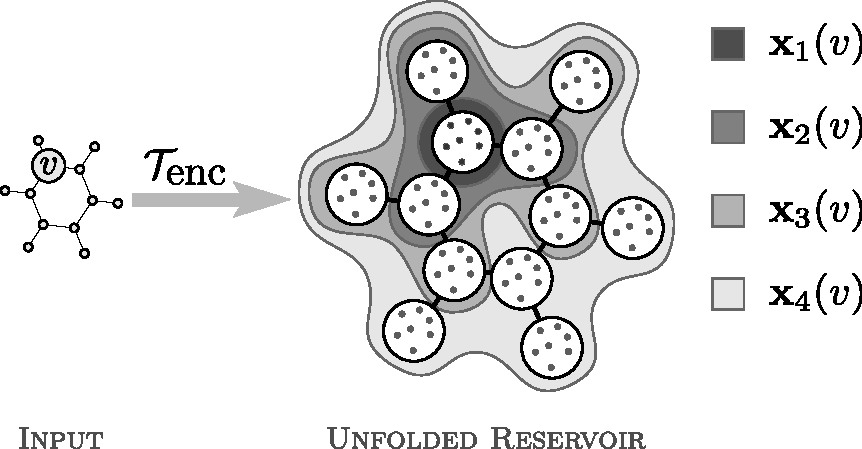
\includegraphics[width=0.7\columnwidth]{img/encoding-v2}
\medskip
\caption[Encoding di una GraphESN.]{Vertici coinvolti nel calcolo di $\vect{x}_t(v)$ durante quattro passi del processo di encoding.}
\label{fig:intro:encoding}
\end{figure}
La figura~\vref{fig:intro:encoding} mostra quali siano i vertici che contribuiscono al calcolo dello stato corrispondente ad un vertice $v$, evidenziando come nel corso di ogni iterazione la ``frontiera'' dei vertici coinvolti si allarghi. \`E bene sottolineare come, nella sua schematizzazione, la figura non renda conto del fatto che uno stesso vertice possa contribuire al calcolo dello stato di $v$ sia direttamente (i.e.\ il vertice appartiene a $\mathcal{N}(v)$) sia in maniera indiretta (i.e.\ per ogni cammino che partendo da $v$ si estenda, vicino dopo vicino ed iterazione dopo iterazione, fino al vertice in questione).

Nel caso di trasduzioni structure-to-element (si veda il paragrafo~\ref{sec:intro:struct:terminologia}) si ricorre ad un'ulteriore funzione $\mathcal{X} : (\R^{N_R})^{\#} \rightarrow \R^{N_R}$, detta \emph{state mapping function}, che applicata al risultato dell'encoding nello spazio strutturato di features restituisce una rappresentazione in uno spazio vettoriale a dimensione fissa per l'intero grafo. In questo caso l'equazione~(\ref{eq:intro:gesn:trasd}) viene dunque decomposta in
\begin{equation}
\mathcal{T} = \mathcal{T}_\textup{out} \circ \mathcal{X} \circ \mathcal{T}_\textup{enc}
\end{equation}
come mostrato dalla figura~\vref{fig:intro:T-enc-X-out}.
\begin{figure}[tbp]
\centering
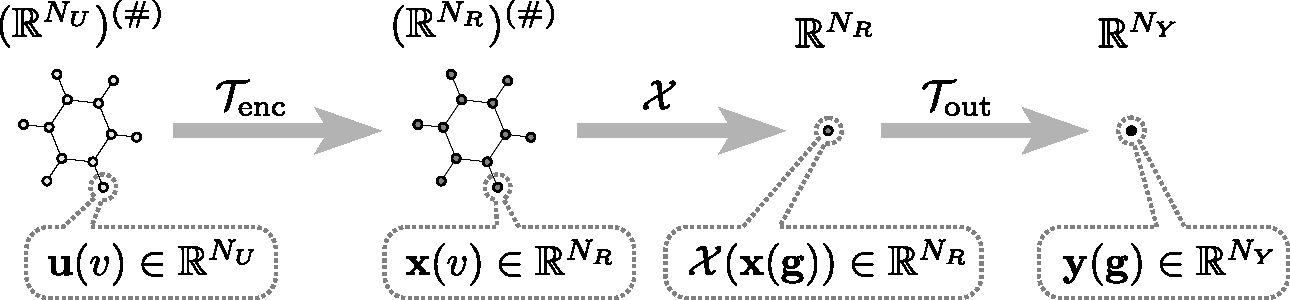
\includegraphics[width=\columnwidth]{img/T-enc-X-out}
\medskip
\caption[Decomposizione di una trasduzione structure-to-element.]{Decomposizione di una trasduzione structure-to-element tramite una funzione di encoding $\mathcal{T}_\textup{enc}$, una state-mapping-function $\mathcal{X}$ ed una funzione di output $\mathcal{T}_\textup{out}$.}
\label{fig:intro:T-enc-X-out}
\end{figure}

Benché la scelta della funzione $\mathcal{X}$ sia arbitraria, si distinguono principalmente due alternative. Con \emph{supersource state mapping} \cite{Gallicchio:TreeESN}, lo stato dell'intero grafo $\mathcal{X}(\vect{x}(\graph{g}))$ viene mappato nello stato di un solo vertice \emph{supersource}, qualora per la natura dei dati o del problema sia individuabile un vertice che dipenda da tutti gli altri\footnote{Questa caratteristica, naturale nel caso di alberi radicati e sequenze, è comunque realizzabile ``artificialmente'' per qualsiasi grafo aggiungendo un vertice che sia collegato a tutti gli altri.}. In alternativa, con \emph{mean state mapping}, $\mathcal{X}(\vect{x}(\graph{g}))$ viene calcolato come la media degli stati corrispondenti ai vertici di $\graph{g}$:
\begin{equation}\label{eq:meanstate}
\mathcal{X}(\vect{x}(\graph{g})) = \dfrac{1}{\abs{V(\graph{g})}} \sum_{v \in V(\graph{g})} \vect{x}(v)
\end{equation}

Come in una ESN, la funzione di output $\mathcal{T}_\textup{out}$ è realizzata da un \emph{readout} formato da $N_Y$ unità che ricevono input dal reservoir (o dalla state mapping function). \\
Nel caso di trasduzioni structure-to-structure, la \emph{funzione di output locale} applicata agli stati corrispondenti ai singoli vertici è la seguente:
\begin{equation}
\vect{y}(v) = g_\textup{out}(\vect{x}(v)) = f_\textup{out}(\matr{W}_\textup{out} \vect{x}(v))
\end{equation}
dove $\vect{y}(v) \in \R^{N_Y}$ è il vettore dei valori di output per il vertice $v$, $\matr{W}_\textup{out} \in \R^{N_Y \times (N_R + 1)}$ è la matrice dei pesi delle connessioni tra reservoir e readout ed $f_\textup{out}$ è la funzione di attivazione delle unità di output, tipicamente lineare. L'applicazione di $g_\textup{out}$ all'encoding ottenuto per ogni vertice dell'input definisce il calcolo della funzione di output $\mathcal{T}_\textup{out}$.\\
Per trasduzioni structure-to-element, l'output a dimensione fissa relativo all'intero grafo, $\vect{y}(\graph{g}) \in \R^{N_Y}$, è invece ottenuto applicando la funzione di output locale al risultato della state mapping function: 
\begin{equation}
\vect{y}(\graph{g}) = g_\textup{out}(\mathcal{X}(\vect{x}(\graph{g})) = f_\textup{out}(\matr{W}_\textup{out} \mathcal{X}(\vect{x}(\graph{g})))
\end{equation}

In entrambi i casi, ed in maniera simile a quanto accade in una ESN standard, l'allenamento di una GraphESN prevede l'adattamento dei pesi della matrice $\matr{W}_\textup{out}$, realizzabile attraverso regressione lineare\footnote{Purché $f_\textup{out}$ sia invertibile, è possibile ricondurre $g_\textup{out}$ ad una combinazione lineare semplicemente modificando i valori target: $\vect{y}_\textup{target}' = f_\textup{out}^{-1}(\vect{y}_\textup{target})$.} sulla base dei valori di target $\vect{y}_\textup{target}(v)$, o $\vect{y}_\textup{target}(\graph{g})$ nel caso di trasduzioni structure-to-element. 

La possibilità di limitare l'apprendimento alla sola funzione di output $g_\textup{out}$ e la realizzazione dell'encoding sfruttando il setting contrattivo del reservoir caratterizzano positivamente le GraphESN dal punto di vista computazionale rispetto ad altri modelli neurali per il trattamento di domini strutturati.\\
Assumendo che il reservoir sia sparso, con $M$ connessioni in input per ogni unità, il costo computazionale di un passo del processo di encoding ha costo
\begin{equation}
O(\abs{V(\graph{g})}\ k\ N_R\ M)
\end{equation}
ed ha dunque una dipendenza lineare sia con il numero di vertici dell'input che con le dimensioni del reservoir. Tale costo risulta molto inferiore, ad esempio, rispetto al processo di encoding realizzato durante la fase di training delle GNN \cite{Scarselli:GNN}, che avviene attraverso centinaia o migliaia di iterazioni, ognuna corrispondente all'intero processo di codifica dell'input di una GraphESN. 
Il costo computazionale dell'encoding è confrontabile anche con metodi basati su kernel applicati al trattamento di grafi. Mantenendo l'assunzione che $k$ sia il grado massimo riscontrabile sul dataset, l'applicazione dell'\emph{optimal assignment kernel} e del \emph{expected match kernel} \cite{Frohlich:AssignmentKernels} risulta infatti avere costo rispettivamente cubico e quadratico rispetto al numero di vertici dell'input.\\
Il costo del trainig varia invece a seconda dell'algoritmo utilizzato, potendo comunque fare affidamento sull'impiego di algoritmi efficienti per l'allenamento di un unico layer di unità feedforward (si veda il paragrafo~\ref{intro:alg}).

La figura~\vref{fig:intro:gesn} riassume schematicamente la struttura ed il funzionamento complessivo di una GraphESN che modelli traduzioni structure-to-element. Procedendo da sinistra verso destra, un grafo in input $\graph{g}$ viene codificato dal reservoir, che lo mappa in uno spazio delle features strutturato. La figura mostra in questo caso l'unfolding del reservoir, che viene ``copiato'' su ogni vertice dell'input. La varie copie così ottenute sono collegate, tramite connessioni con pesi in $\hat{\matr{W}}$, in accordo alla topologia del grafo (i.e.\ in base ai vicini di ogni vertice). Successivamente l'encoding ottenuto viene trasformato, dalla state mapping function $\mathcal{X}$, in un vettore di features a dimensione fissa. Il risultato dell'applicazione della state mapping function viene infine usato come input del readout, unica componente adattiva del modello, ottenendo in output il vettore a dimensione fissa $\vect{y}(\graph{g})$. In alto a sinistra la figura mostra la dipendenza che lega gli stati nello spazio delle features, sia all'etichetta di input del vertice corrispondente che agli stati calcolati in corrispondenza dei suoi vicini (i.e.\ un unico vicino nella figura).

\begin{figure}[tbp]
\centering
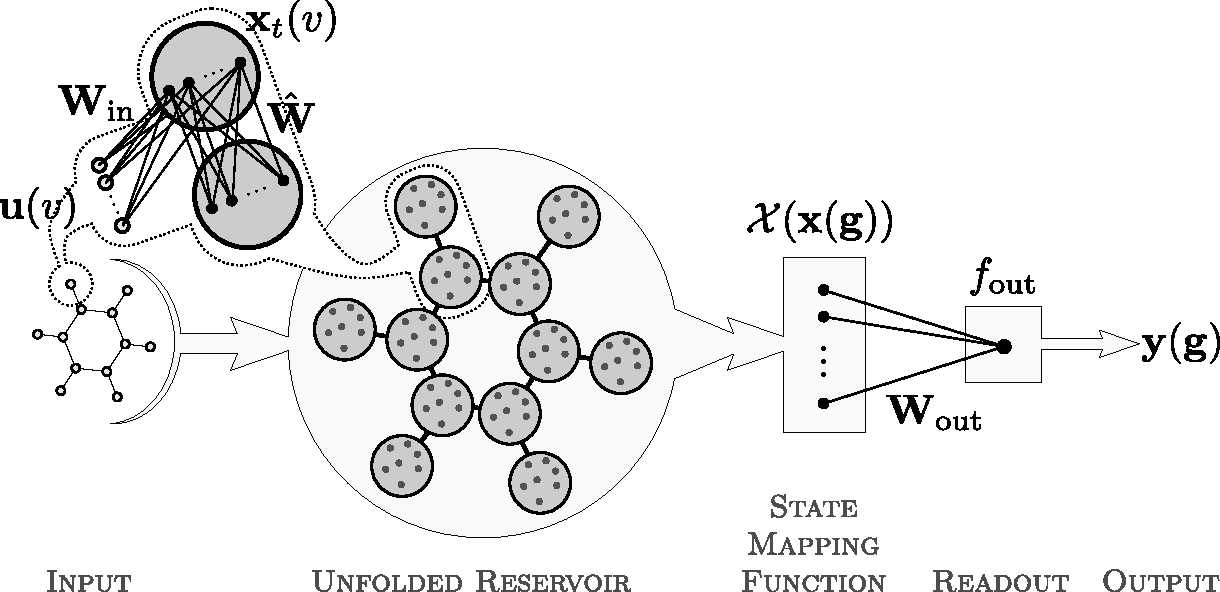
\includegraphics[width=0.95\columnwidth]{img/GraphESN-v2}
\medskip
\caption[GraphESN.]{Schema di una GraphESN per l'apprendimento di trasduzioni structure-to-element.}
\label{fig:intro:gesn}
\end{figure}

